\chapter{First run}

In this chapter we show the usage of Pepr3D for complete beginners. It covers every step from starting Pepr3D to exporting simple colored model including importing, manipulating and using tools.


\section{First look at Pepr3D}

When you run Pepr3D, you will see a cube at the center of the application. There is a toolbar at the top of application which contains file menu, undo/redo buttons, set of tools and some settings. There is also a side pane on the right with settings of individual tools as you can see in figure \ref{fig:pepr_cube}.

\begin{figure}
	\centering
	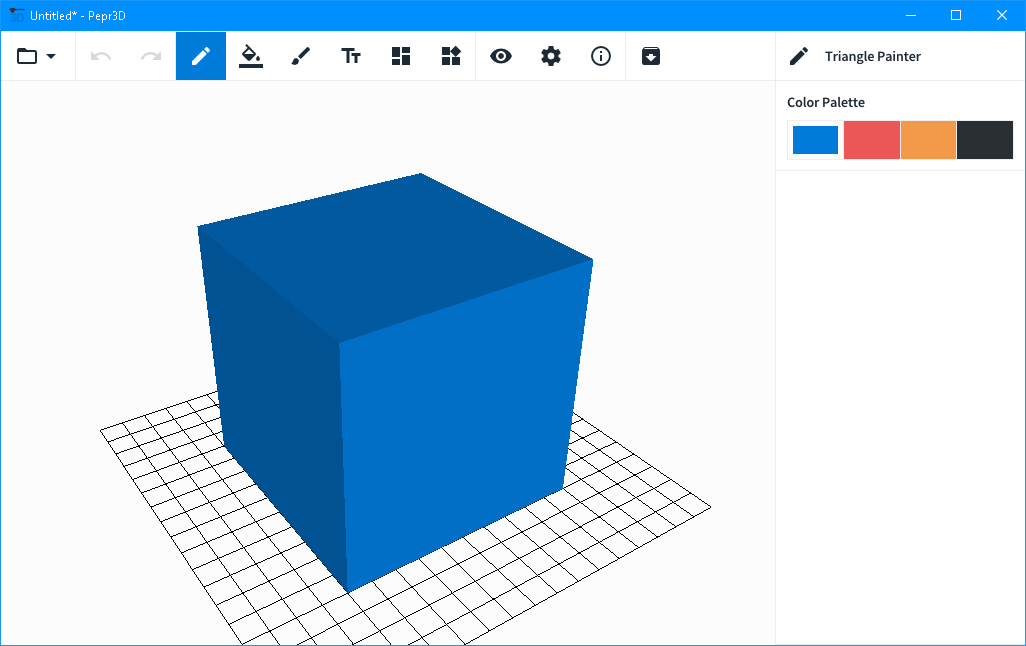
\includegraphics[scale=0.5]{images/pepr_cube.png}
	\caption{Pepr3D appearance after startup.}
	\label{fig:pepr_cube}
\end{figure}

\subsection{Model manipulation}
You can manipulate the model by using your mouse. There are several ways to manipulate so you can reach and see any part of the model:

\begin{itemize}
\item \textbf{Rotation} -- click and hold right mouse button and move.
\item \textbf{Translation} -- press Ctlr + right mouse button and move or click and hold middle mouse button (mouse wheel) and move the mouse.
\item \textbf{Zoom} -- rotate mouse wheel.
\end{itemize}

Left mouse button is dedicated to using selected tool.

\section{First model}
Now we can start working on a simple model with Pepr3D. First we have to acquire a 3D model, it should be in one of these file formats: \texttt{.stl}, \texttt{.ply}, \texttt{.obj}. Simplest way to acquire model is choose any model on the Internet and download it. Or you can use any 3D modeling software and create your own one. In this tutorail we use simple low-polygon model of Bulbasaur downloaded from Thingiverse\footnote{https://www.thingiverse.com/thing:327753}.

To import the model we can use drag and drop gesture with model file or we can browse for model file after clicking \textit{Import} in file menu.


\subsection{Painting the model}

After importing the model we can use any tool that our application provides to color the model as we want. In a few steps, we will show how to quickly color the imported model of Bulbasaur with basic tools.

\begin{enumerate}
\item Select \textit{Triangle Painter} tool, choose black color.
\item Paint all triangles in each eye by clicking on them with left mouse button. It is possible to click and drag to paint multiple adjacent triangles.
\item Use the same technique and paint its ears.

\begin{center}
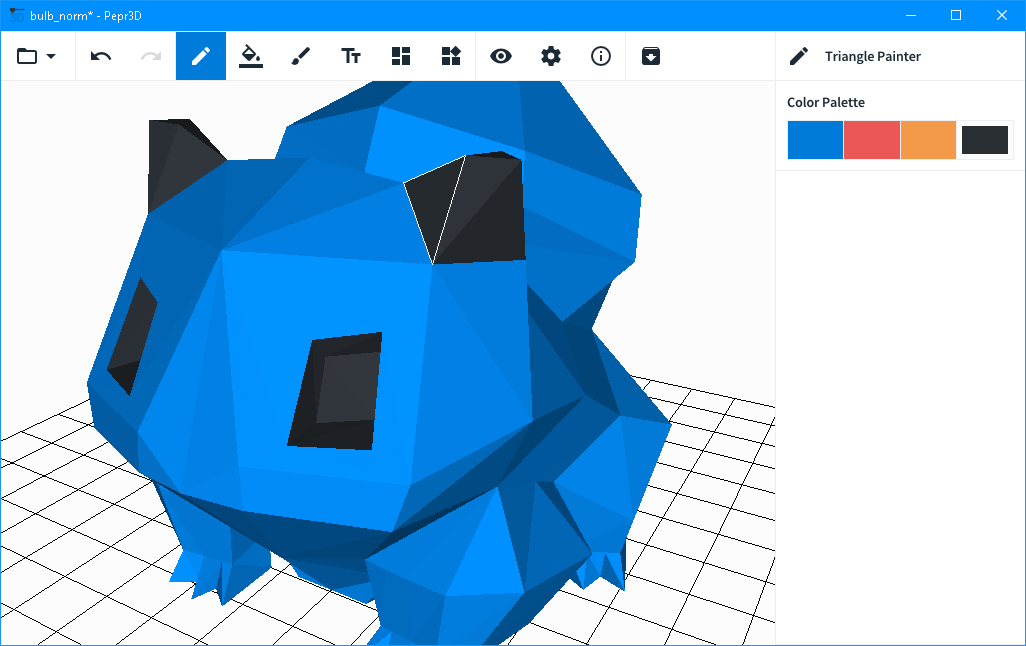
\includegraphics[scale=0.4]{images/bulb_eyes.png}
\end{center}

\item Choose another color (red) and select \textit{Paint Bucket} tool.
\item Check \textit{Stop on sharp edges} in side pane and set \textit{Maximum angle} to 45$^\circ$.
\item Use \textit{Paint Bucket} on any triangle on an "onion" on the back of the Bulbasaur. Click two more times on any unpainted triangle to paint whole "onion" with red color.
\item Select \textit{Triangle Painter} and first color (blue) and recolor two triangles near neck which have been painted extra by \textit{Paint Bucket} in previous step.

\begin{center}
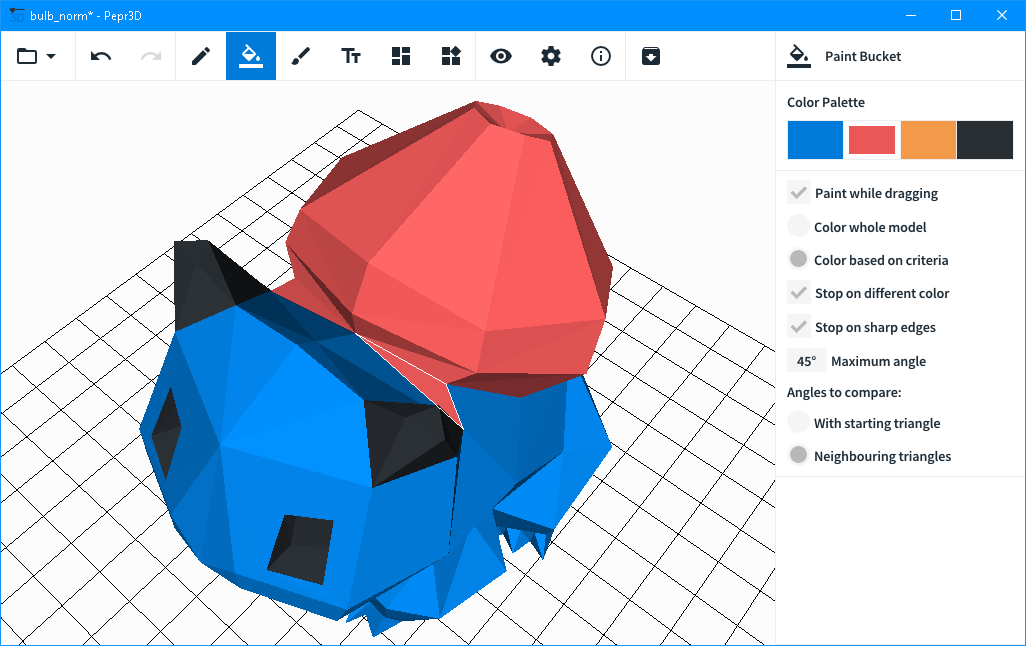
\includegraphics[scale=0.4]{images/bulb_onion.png}
\end{center}

\item Select \textit{Brush} tool and check \textit{Respect original triangles} and also check \textit{Paint outer ring} in the settings of the tool.
\item Set brush size to about 4.0.
\item Choose orange and paint all its legs. Do not forget to paint the legs from below.

\begin{center}
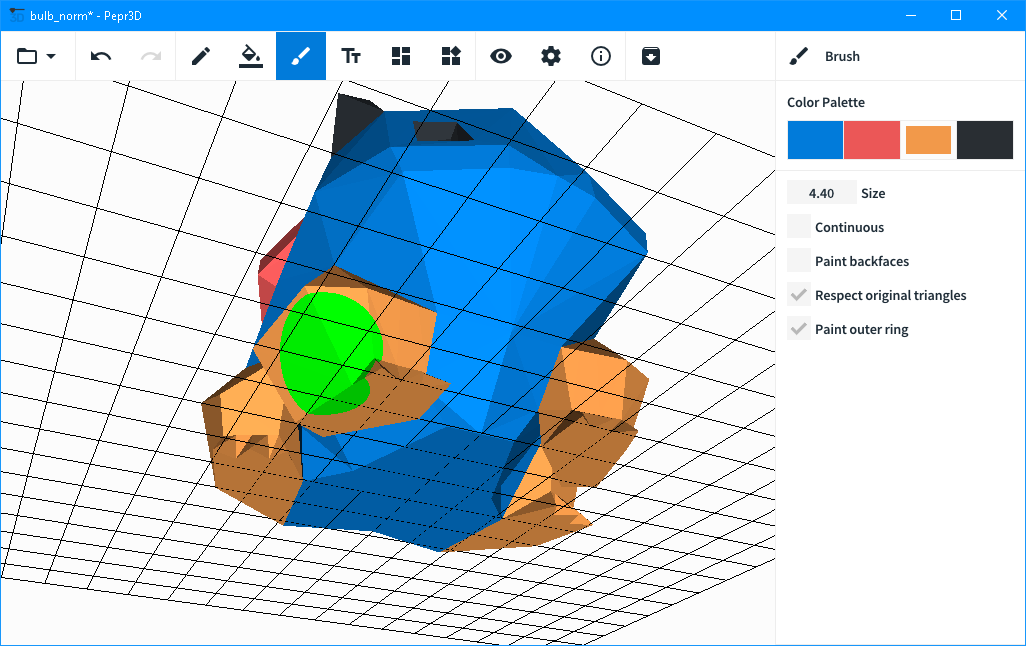
\includegraphics[scale=0.4]{images/bulb_legs.png}
\end{center}

\end{enumerate}


You can undo any step you did with any tool. For example, if you paint incorrect triangle, you can press \textit{Undo} (left arrow) in toolbar for reverting last action.

\subsection{Exporting the model}
Now the model is painted and we can proceed to model exporting. Before exporting the model itself we need to set depth of color extrusion into the model. Exporting tutorial can be summarized in following steps:


\begin{enumerate}
\item Open \textit{Export Assistant} on the toolbar or click \textit{Export} in file menu.
\item Click \textit{Update extrusion preview!} button.
\item Lower percentage of \textit{Max Preview height} to see into the model and see the thickness of model walls -- extrusion depth.
\item Adjust the percentage of \textit{Depth} for desired extrusion depth.
\item Update preview by clicking on \textit{Update extrusion preview!}.
\item Repeat adjusting the depth and updating preview until satisfaction.
\item Click on \textit{Export files} and complete the export.
\end{enumerate}

\begin{figure}
	\centering
	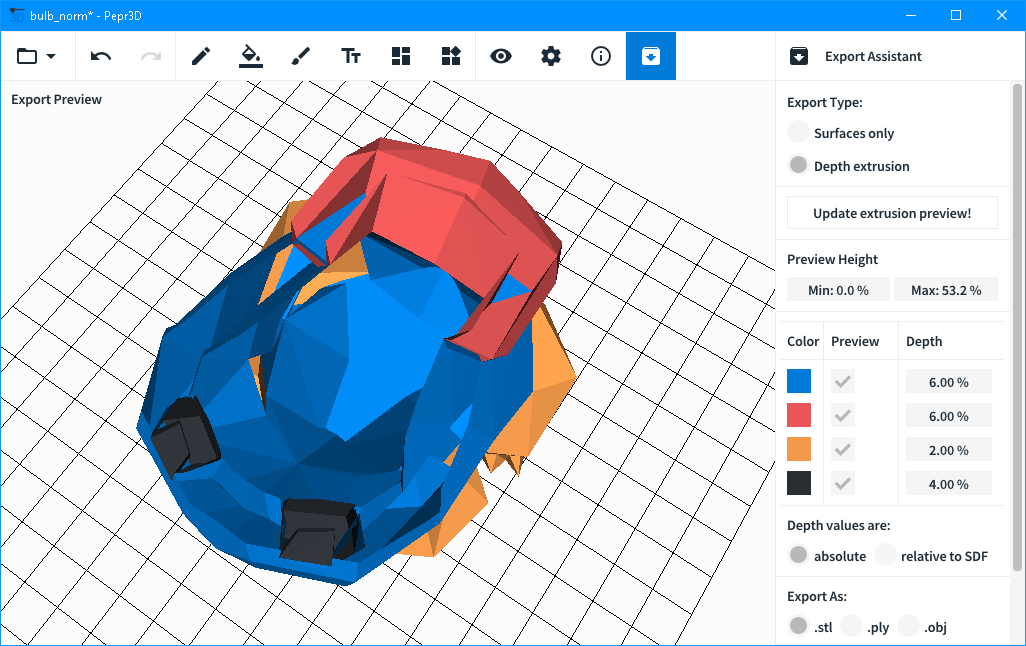
\includegraphics[scale=0.5]{images/bulb_export.png}
	\caption{Example of \textit{Export Assistant} with colored model.}
	\label{fig:bulb_export}
\end{figure}


Exported files can be now imported into slicer and printed on multimaterial 3D printer.




